\section{3D Gaussian Splatting and Surface Reconstruction}

Our method relies on the original 3D Gaussian Splatting~(3DGS) method~\cite{kerbl3Dgaussians} for initialization and on SuGaR~\cite{guedon2023sugar} to align Gaussians with the surface of the scene and facilitate the extraction of a mesh. We briefly describe 3DGS and SuGaR in this section before describing our method in the next section.


\subsection{3D Gaussian Splatting} 

3DGS represents the scene as a large set of Gaussians. Each Gaussian $g$ is equipped with a mean $\mu_g\in \IR^3$ and a positive-definite covariance matrix $\Sigma_g\in \IR^{3\times 3}$. The covariance matrix is parameterized by a scaling vector $s_g\in\IR^3$ and a quaternion $q_g\in\IR^4$ encoding the rotation of the Gaussian. 

In addition, each Gaussian has a view-dependent radiance represented by an opacity $\alpha_g\in [0,1]$ and a set of spherical harmonics coordinates defining the colors emitted for all directions. To render an image from a given viewpoint, a rasterizer ``splats'' the 3D Gaussians into 2D Gaussians parallel to the image plane and blends the splats depending on their opacity and depth. This rendering is extremely fast, which is one of the advantages of 3DGS over volumetric rendering as in NeRFs for example~\cite{mildenhall2020nerf, mueller2022instantngp, barron2022mipnerf360}.


Gaussian Splatting can be seen as an approximation of the traditional volumetric rendering of radiance fields with the following density function $d$, computed as the sum of the Gaussian values weighted by their alpha-blending coefficients at any 3D point $p\in \IR^3$:
%
 \begin{equation}
    d(p) = \sum_{g} \alpha_g \exp\left(-\frac{1}{2}(p - \mu_g)^T \Sigma^{-1}_g (p - \mu_g)\right) \> .
    \label{eq:gaussian_splatting_density}
\end{equation}

We initialize our Gaussian Frosting method using a vanilla 3DGS optimization: Gaussians are initialized using the point cloud produced by an SfM~\cite{snavely-2006-structure-from-motion} algorithm like COLMAP~\cite{schoenberger2016mvs,schoenberger2016sfm}, required to compute camera poses. The Gaussians' parameters (3D means, scaling vectors, quaternions, opacities, and spherical harmonics coordinates) are then optimized to make the renderings match the ground truth images of the scene, using a rendering loss that only consists in a combination of a pixel-wise L1 distance and a more structural D-SSIM term. 


\subsection{SuGaR Mesh Extraction} 

Vanilla 3DGS does not have regularization explicitly encouraging Gaussians to align with the true surface of the scene. Our Gaussian Frosting representation relies on a mesh that approximates this surface, in order to be editable by traditional tools. To obtain this mesh, we rely on the method proposed in SuGaR~\cite{guedon2023sugar}, which we improve by automatically selecting a critical hyperparameter.

SuGaR proposes a regularization term encouraging the alignment of the 3D Gaussians with the true surface of the scene during the optimization of Gaussian Splatting, as well as a mesh extraction method. After enforcing the regularization, the optimization provides Gaussians that are mostly aligned with the surface albeit not perfectly: We noticed that in practice, a large discrepancy between the regularized Gaussians and the extracted mesh indicates the presence of fuzzy materials or surfaces that require volumetric rendering. We thus exploit this discrepancy as a cue to evaluate where the Frosting should be thicker.

\begin{figure}[tb]
  \centering
  % 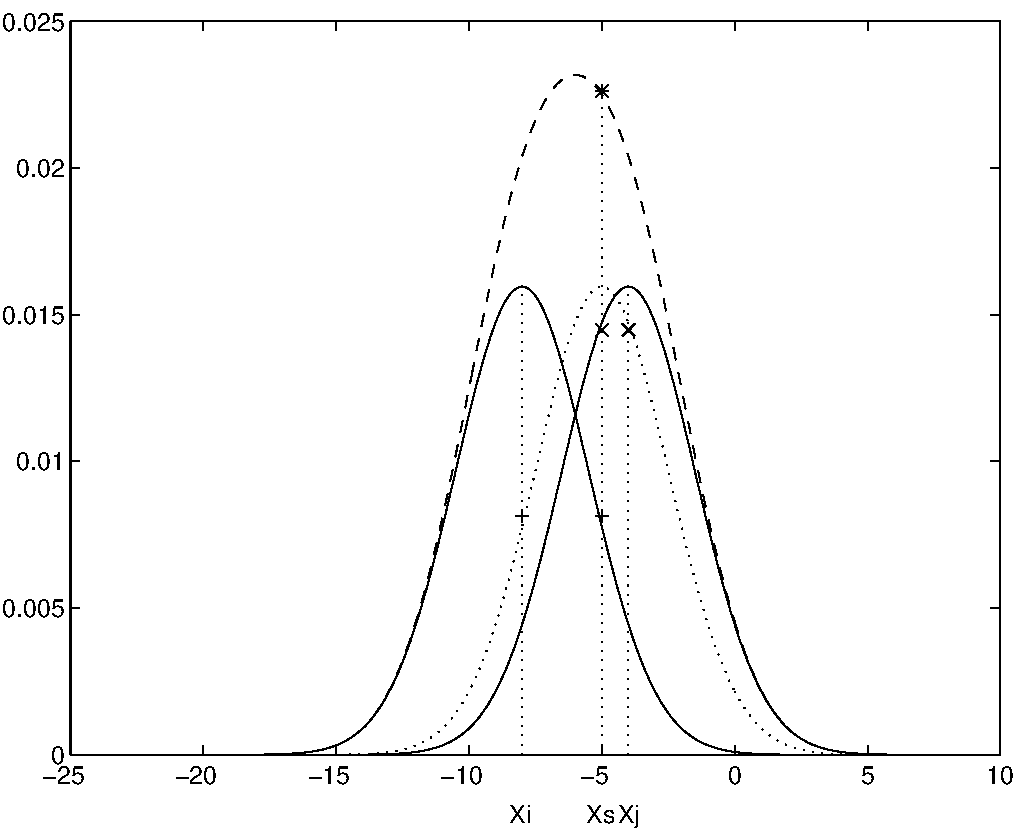
\includegraphics[height=6.5cm]{eijkel2}
  % \fbox{\rule{0pt}{0.8in} \rule{.95\linewidth}{0pt}}
  %\includesvg[inkscapelatex=false, width = 1\linewidth]{images/pipeline_frosting_largefont}
  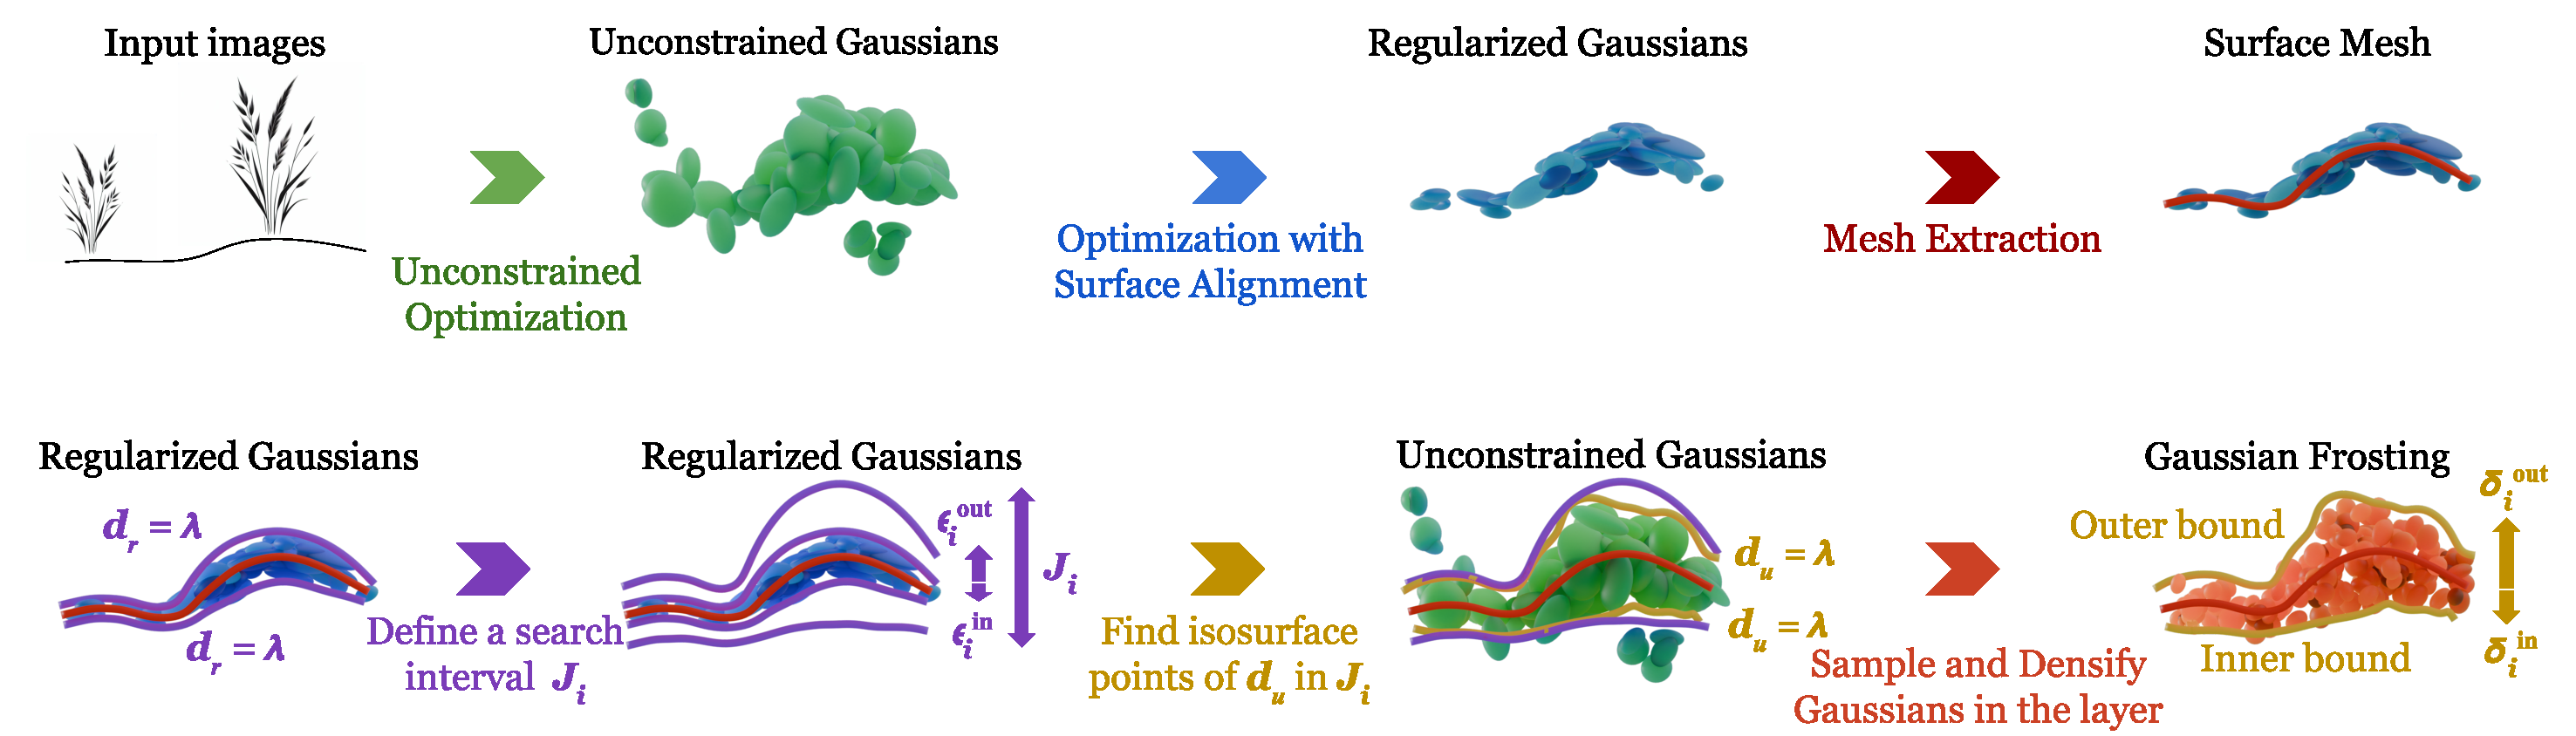
\includegraphics[width=\linewidth]{images/pipeline_frosting_largefont.pdf}
  \caption{
  \textbf{Creating a Layer of Gaussian Frosting.} To build our proposed Frosting representation, we start by optimizing a Gaussian Splatting representation using a rendering loss without any additional constraint, to let Gaussians position themselves. We refer to these Gaussians as \emph{unconstrained}. We then regularize these Gaussians to enforce their alignement with the surface, and extract a mesh that will serve as a basis for the Frosting. Next, we use the misalignment of surface-aligned Gaussians to identify areas where more volumetric rendering is needed, and we build search intervals $J_i$ around the mesh's vertices $\vec{v_i}$. Finally, we use the density function of the unconstrained Gaussians to refine the intervals, resulting in a Frosting layer. We finally sample a novel, densified set of Gaussians inside the layer.
}
  \label{fig:frosting-pipeline}
\end{figure}

\section{Creating a Frosting Layer from Images}

In this section, we describe our Gaussian Frosting creation method: 
First, we extract an editable surface with optimal resolution using SuGaR. We then detail how we use this surface-based model to go back to a volumetric but editable representation built around the mesh. This representation adapts to the complexity of the scene and its need for more volumetric effects. Finally, we describe how we parameterize and refine this representation. An overview is provided Figure~\ref{fig:frosting-pipeline}.

\subsection{Forward Process: From Volume to Surface}
\label{subsec:forward-process}

We start by optimizing an unconstrained Gaussian Splatting representation for a short period of time to let Gaussians position themselves. We will refer to such Gaussians as \emph{unconstrained}. We save these Gaussians aside, and apply the regularization term from SuGaR to enforce the alignment of the Gaussians with the real surface. We will refer to these Gaussians as \emph{regularized}.

Once we obtain the regularized Gaussians, we extract a surface mesh from the Gaussian Splatting representation. This surface mesh serves as a basis for our representation. Like SuGaR~\cite{guedon2023sugar}, we then sample points on the visible level set of the Gaussian splatting density function, and apply Poisson reconstruction. 

In the supplementary material, we describe our technique to automatically estimate a good value for a critical hyperparameter used by Poisson reconstruction, namely the octree depth $D$. As we will show in the Experiments section, selecting the right value for $D$ when applying Poisson reconstruction can drastically improve both the quality of the mesh and the rendering performance of our model. Figure~\ref{fig:mesh-comparison} illustrates this point.


\begin{figure}[tb]
  \centering
  \begin{subfigure}{0.19\linewidth}
  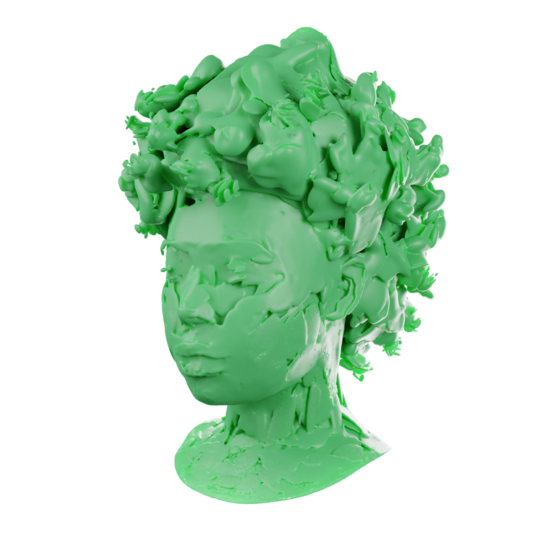
\includegraphics[width=\linewidth]{images/meshes/khady_sugar.png}
  \end{subfigure}
  %
  \hfill
  %
  \begin{subfigure}{0.19\linewidth}
  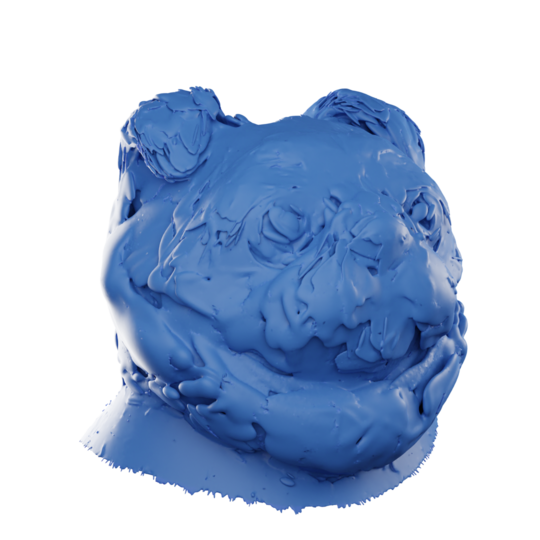
\includegraphics[width=\linewidth]{images/meshes/pug_sugar.png}
  \end{subfigure}
  %
  \hfill
  %
  \begin{subfigure}{0.19\linewidth}
  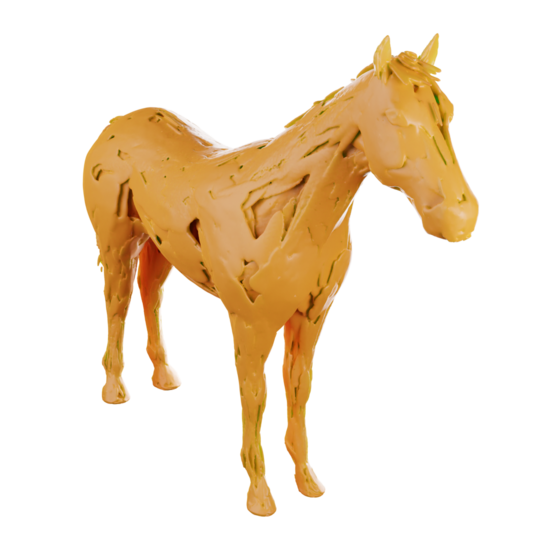
\includegraphics[width=\linewidth]{images/meshes/horse_y_sugar.png}
  \end{subfigure}
  %
  \hfill
  %
  \begin{subfigure}{0.19\linewidth}
  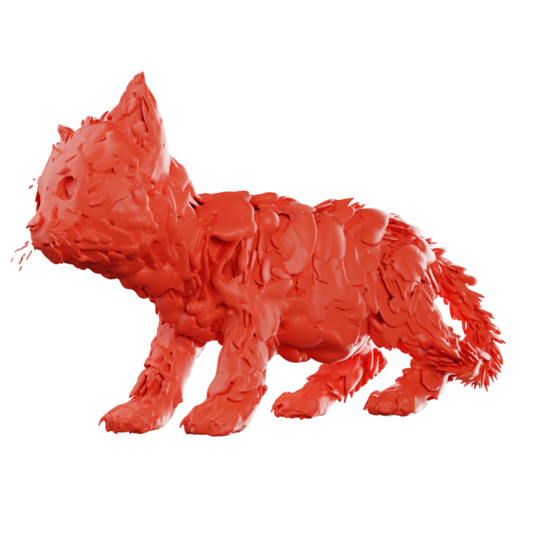
\includegraphics[width=\linewidth]{images/meshes/kitten_sugar.png}
  \end{subfigure}
  %\hfill
  %
  % \begin{subfigure}{0.19\linewidth}
  % \includegraphics[width=\linewidth]{images/meshes/woolly_sugar.png}
  % \end{subfigure}
  %
  %
  \vspace{0.005\linewidth}\\
  {\small (a) Using the predefined, large parameter $D$ as in SuGaR~\cite{guedon2023sugar}} 
  % \vspace{0.01\linewidth}
  \\
  %
  \begin{subfigure}{0.19\linewidth}
  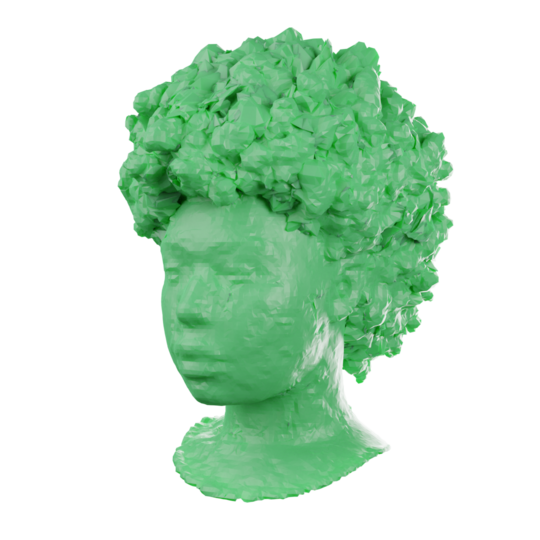
\includegraphics[width=\linewidth]{images/meshes/khady_frosting.png}
  \end{subfigure}
  %
  \hfill
  %
  \begin{subfigure}{0.19\linewidth}
  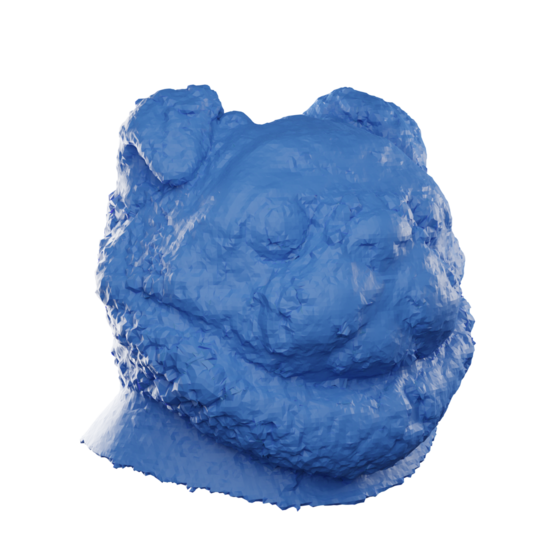
\includegraphics[width=\linewidth]{images/meshes/pug_frosting.png}
  \end{subfigure}
  %
  \hfill
  %
  \begin{subfigure}{0.19\linewidth}
  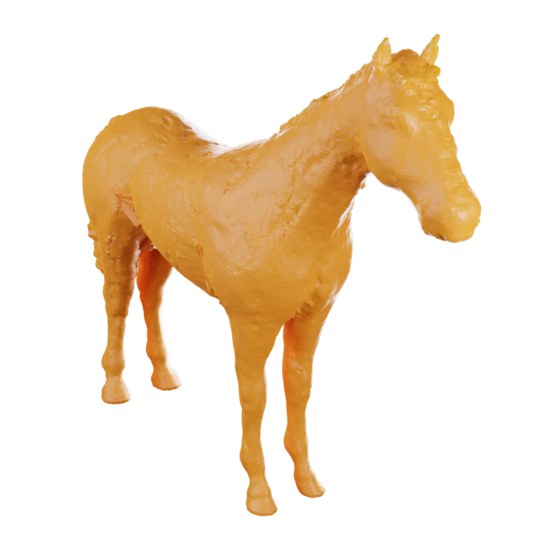
\includegraphics[width=\linewidth]{images/meshes/horse_y_frosting.png}
  \end{subfigure}
  %
  \hfill
  %
  \begin{subfigure}{0.19\linewidth}
  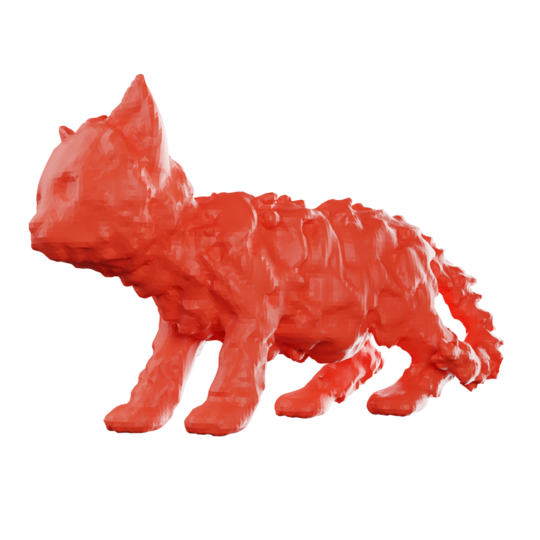
\includegraphics[width=\linewidth]{images/meshes/kitten_frosting.png}
  \end{subfigure}
  %
  % \hfill
  % %
  % \begin{subfigure}{0.19\linewidth}
  % \includegraphics[width=\linewidth]{images/meshes/woolly_frosting.png}
  % \end{subfigure}
  %
  % \vspace{0.005\linewidth}
  \\
  {\small (b) Using our automatically computed $D$ that adapts to the complexity of the 3DGS}
  %
  \caption{
  \textbf{Comparison of meshes extracted by SuGaR from the Shelly dataset without and with our improvement that automatically tunes the octree depth $D$ in Poisson reconstruction depending on the complexity of the scene.}
  Our technique~(bottom) drastically reduces surface artifacts for many scenes, such as the holes and the ellipsoidal bumps on the surface when using the default values from~\cite{guedon2023sugar}~(top).
}
  % \vincentrmk{I would remove the purple thing on the right, the 2 meshes are not very different}
%  \vincentrmk{I removed the wooly thing}
  % Moreover, the outer bound of the frosting layer~(bottom), which is computed using the unconstrained, non-aligned Gaussians, generally provides a refined mesh with better quality than the mesh directly obtained from the isosurface of the aligned Gaussians.
  
  
    % \textbf{Comparison of meshes reconstructed from Gaussian Splatting representations using SuGaR~\cite{guedon2023sugar} and our approach.}
  % Our method to compute automatically optimal hyperparameters for Poisson recontruction~(center) drastically reduces surface artifacts for a lot of scenes, such as the ellipsoidal bumps on the surface when using the default values from~\cite{guedon2023sugar}~(left). Moreover, the outer bound of the frosting layer~(right), which is computed using the unconstrained, non-aligned Gaussians, generally provides a refined mesh with better quality than the mesh directly obtained from the isosurface of the aligned Gaussians.}}
  \label{fig:mesh-comparison}
\end{figure}
% \todo{We also follow SuGaR~\cite{guedon2023sugar} for extracting a base mesh, but we can actually give more details as shown above. Indeed, SuGaR is very elusive on this part; I think it's interesting to understand what Poisson reconstruction provides, that the density functions lacks. Moreover, this part may be important to explain the improvement that I a added, which is a way to automatically compute the optimal octree depth hyperparameter for Poisson reconstruction depending on the configuration of the Gaussians in the scene. This greatly helps to remove "blobs" in the scene without having to tweak the octree depth parameter by hand, so it could be a contribution. Having a well-balanced mesh is important to get a nice frosting.}


\subsection{Backward Process: From Surface to Volume}
\label{sec:shifts}

After extracting a base mesh, we build a Frosting layer with a variable thickness and containing Gaussians around this mesh. We want this layer to be thicker in areas where more volumetric rendering is necessary near the surface, such as fuzzy material like hair or grass for example. On the contrary, this layer should be very thin near the parts of the scene that corresponds to well-defined flat surfaces, such as wood or plastic for example.

\begin{figure}[t]
  \centering
  % \includesvg[inkscapelatex=false, width = 1\linewidth]{images/ray.svg}
  % \includesvg[inkscapelatex=false, width = 1\linewidth]{images/ray.svg}
  % \includesvg[inkscapelatex=false, width = 1\linewidth]{images/ray_w_mesh.svg}
  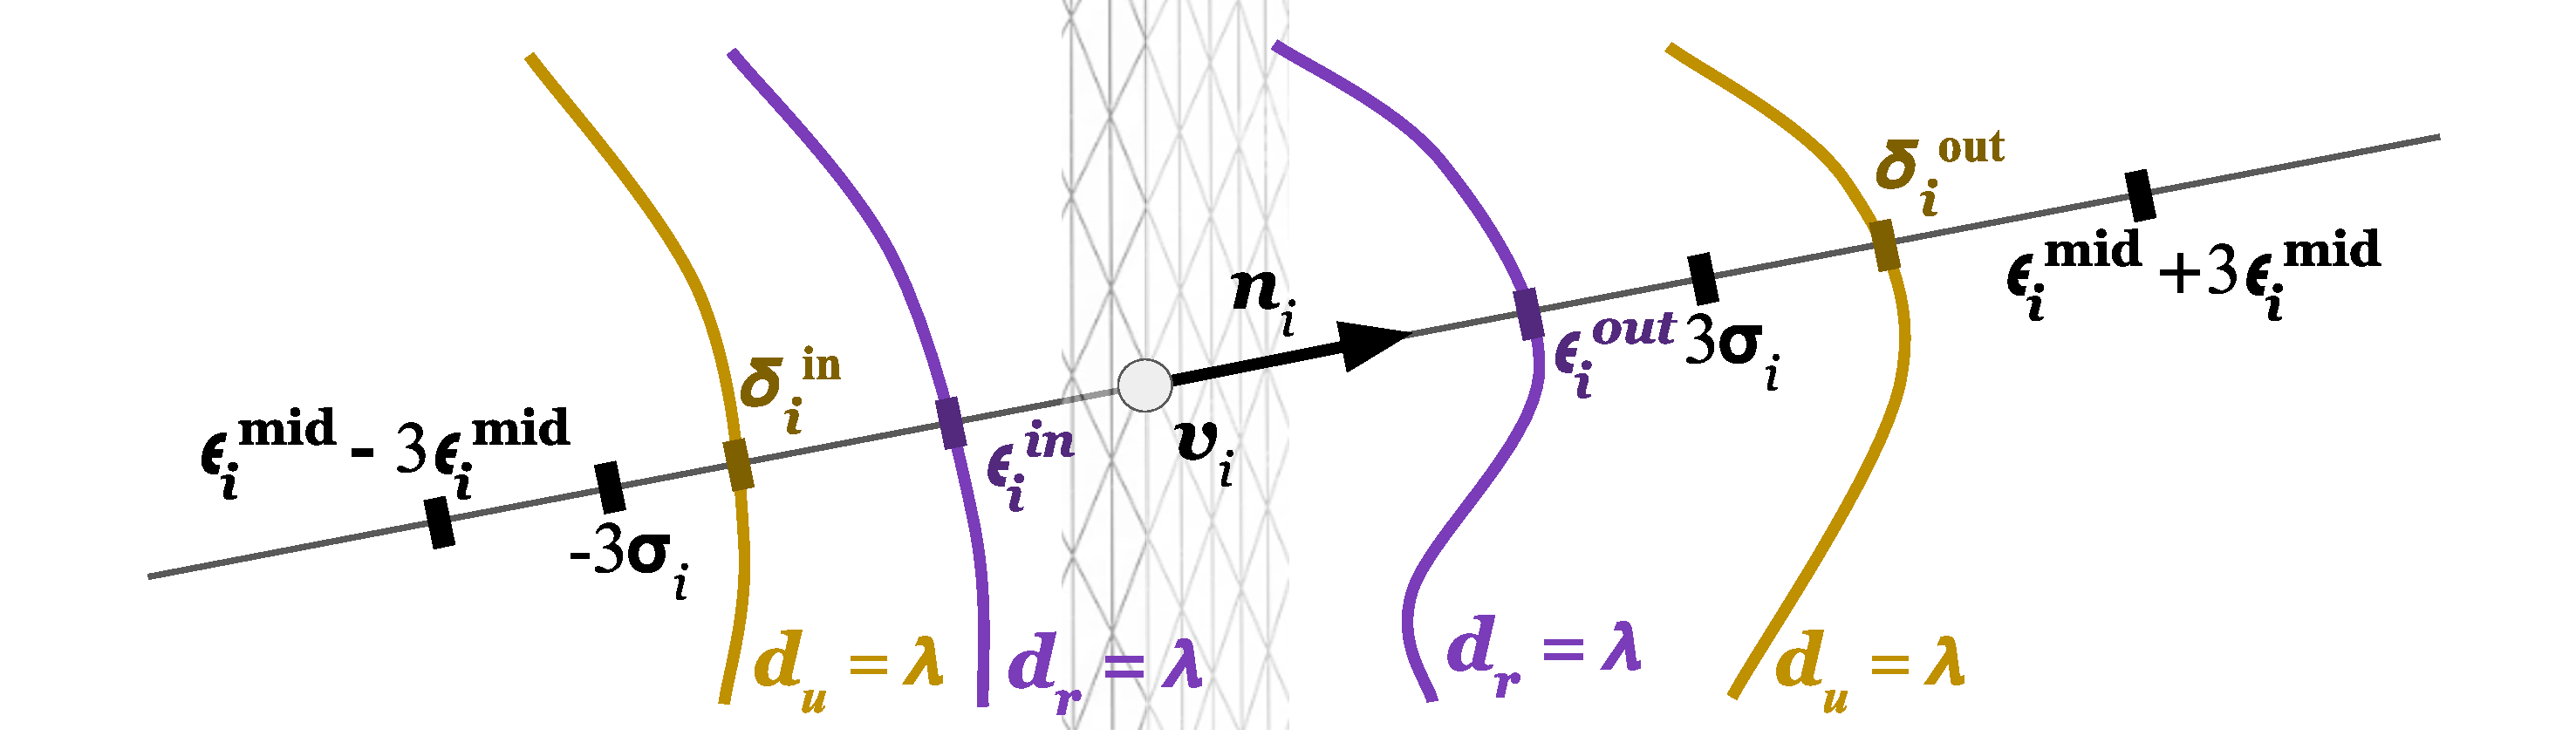
\includegraphics[width=\linewidth]{images/ray_w_mesh.pdf}
  \caption{
  \textbf{How we define the inner and outer bounds of the Frosting layer.} See text in Section~\ref{sec:shifts}.}
  \label{fig:shifts}
\end{figure}


As illustrated in Figure~\ref{fig:shifts}, to define this layer, we introduce two values $\innershift_i$ and $\outershift_i$ for each vertex $\vec{v}_i$ of the extracted base mesh $\calM$. This gives two surfaces with vertices $(\vec{v}_i+\innershift_i \vec{n}_i)_i$ and $(\vec{v}_i+\outershift_i \vec{n}_i)_i$ respectively, where $\vec{n}_i$ is the mesh normal at vertex $\vec{v}_i$. These two surfaces define the inner and outer bounds of the Frosting layer. Note that we do not have to build them explicitly as they directly depend on the base mesh and the $\innershift_i$'s and $\outershift_i$'s.


To find good values for the $\innershift_i$'s and $\outershift_i$'s, we initially tried using directly the unconstrained Gaussians, i.e., the Gaussians obtained before applying the regularization term from SuGaR.  Unfortunately, without regularization, Gaussian Splatting tends to retrieve a thick layer of Gaussians even for ``non-fuzzy'' surfaces, which would result in excessively large values for $\innershift_i$ and $\outershift_i$.  Moreover, the unconstrained Gaussians generally contain many transparent floaters and other outlier Gaussians. Such Gaussians could also bias the shifts toward unnecessarily large values. On the other hand, using only the regularized Gaussians to setup the $\innershift_i$'s and $\outershift_i$'s could miss fuzzy areas since these Gaussians are made flatter by the regularization.


Our solution is thus to consider both the unconstrained and the regularized Gaussians.  More exactly, we estimate the Frosting thickness from the thickness of the unconstrained Gaussians by looking for their isosurfaces, BUT, to make sure we consider the isosurfaces close to the scene surface, we search for the isosurfaces close to the regularized Gaussians: Even under the influence of the regularization term from SuGaR, Gaussians do not align well with the geometry around surfaces with fuzzy details.  As a consequence, the local thickness of the regularized Gaussians is a cue on how fuzzy the material is.


Figure~\ref{fig:shifts}  illustrates what we do to fix the $\innershift_i$'s and $\outershift_i$'s. To restrict the search, we define a first interval $I_i = [-3\sigma_i, 3\sigma_i]$ for each vertex $\vec{v}_i$, where $\sigma_i$ is the standard deviation in the direction of $\vec{n}_i$ of the regularized Gaussian the closest to $\vec{v}_i$. $I_i$ is the confidence interval for the 99.7 confidence level of the 1D Gaussian function of $t$ along the normal. Fuzzy parts result in general in large $I_i$. We could use the $I_i$'s to restrict the search for the isosurfaces of the unconstrained Gaussians. A more reliable search interval $J_i$ is obtained by looking for the isosurfaces of the regularized Gaussians along  $\vec{n}_i$ within $I_i$:
%
\begin{equation}
    \propinnershift_i = \inf ( T ) \text{ , }
    \propoutershift_i = \sup ( T ) \text{ , with }
    T = \left\{ t\in I_i \>\> | \>\> d_r(\vec{v}_i+t\vec{n}_i) \geq \lambda \right\} \> ,
    \label{eq:proposal-shifts}
\end{equation}
%
where $d_r$ is the density function as defined in Eq.~\eqref{eq:gaussian_splatting_density} for the regularized Gaussians.  In practice, we use an isosurface level~$\lambda = 0.01$, i.e., close to zero.
%
We use $ \propinnershift_i$ and $\propoutershift_i$ to define interval $J_i$: $J_i = \left[ \epsilon^\Mid_i - k\epsilon^\half_i, \epsilon^\Mid_i + k\epsilon^\half_i \right]$, with $\epsilon^\Mid_i = (\propinnershift + \propoutershift)/2$ and $\epsilon^\half_i = (\propoutershift - \propinnershift)/2$. We take $k=3$ as it gives an interval large enough to include most of the unconstrained Gaussians while rejecting the outlier Gaussians. Finally, we can compute the inner and outer shifts~$\innershift_i$ and $\outershift_i$ as:
%
\begin{equation}
    \innershift_i = \inf ( V ) \text{ , }
    \outershift_i = \sup ( V ) \text{ , with }
    V = \left\{ t\in J_i \>\> | \>\> d_u(\vec{v}_i+t\vec{n}_i) \geq \lambda \right\} \> .
    \label{eq:shifts}
\end{equation}

\begin{figure}[tb]
  \centering
  \begin{subfigure}{0.155\linewidth}
  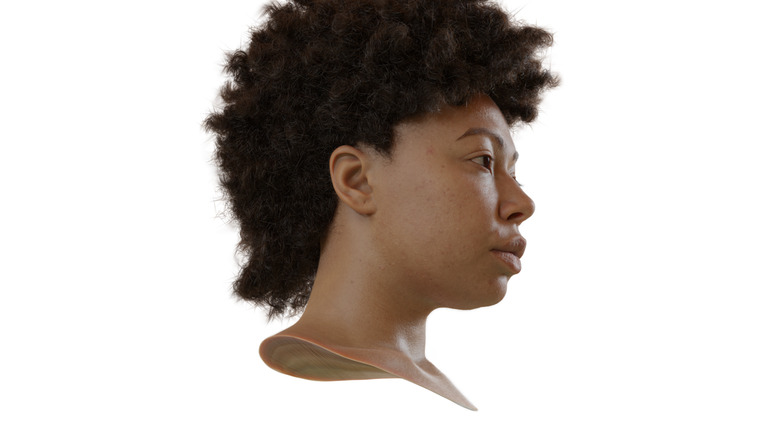
\includegraphics[width=\linewidth]{images/renders/khady_rgb_31.jpg}
  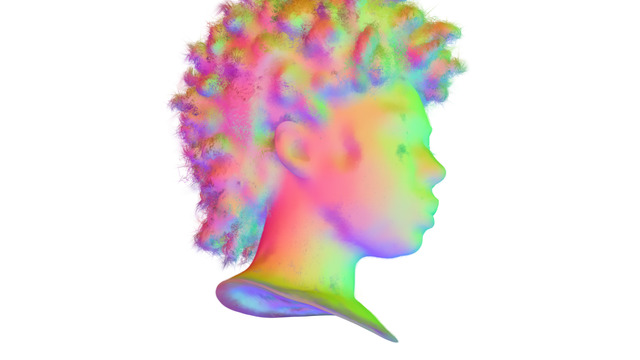
\includegraphics[width=\linewidth]{images/normals/khady_normals_31.jpg}
  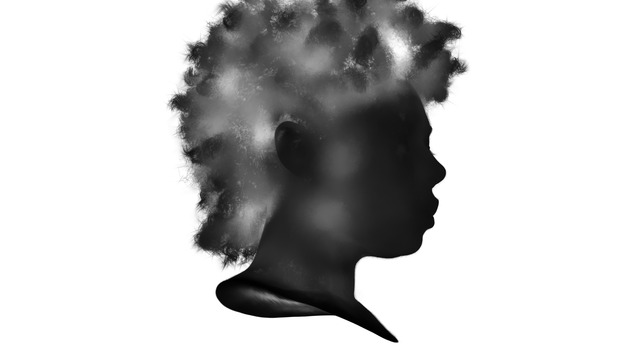
\includegraphics[width=\linewidth]{images/frosting_size/khady_size_31.jpg}
  \end{subfigure}
  %
  \hfill
  %
  \begin{subfigure}{0.155\linewidth}
  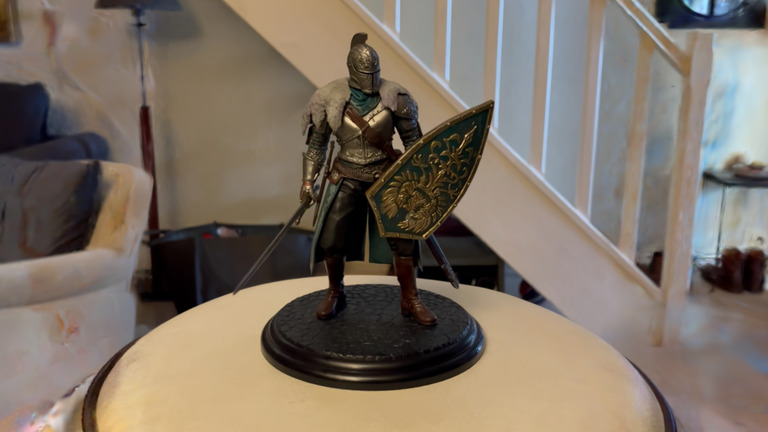
\includegraphics[width=\linewidth]{images/renders/faraam0_rgb_14.jpg}
  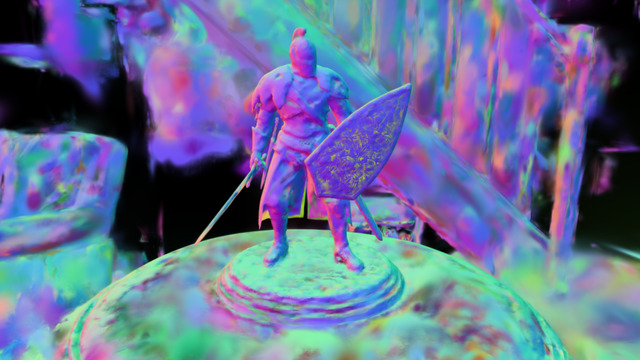
\includegraphics[width=\linewidth]{images/normals/faraam0_normals_14.jpg}
  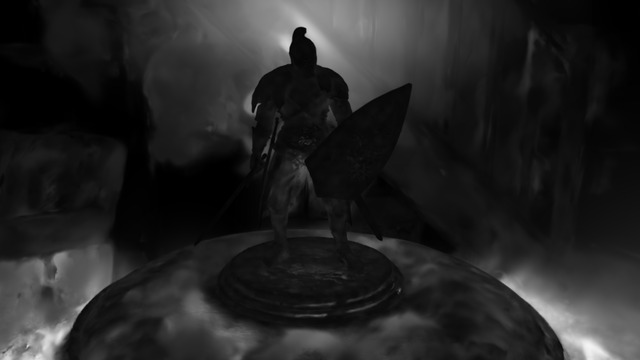
\includegraphics[width=\linewidth]{images/frosting_size/faraam0_size_14.jpg}
  \end{subfigure}
  %
  \hfill
  %
  \begin{subfigure}{0.155\linewidth}
  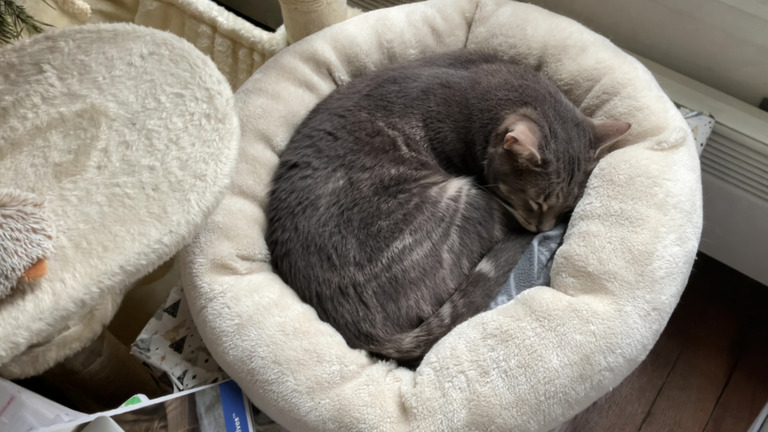
\includegraphics[width=\linewidth]{images/renders/sirius1_rgb_52bis.jpg}
  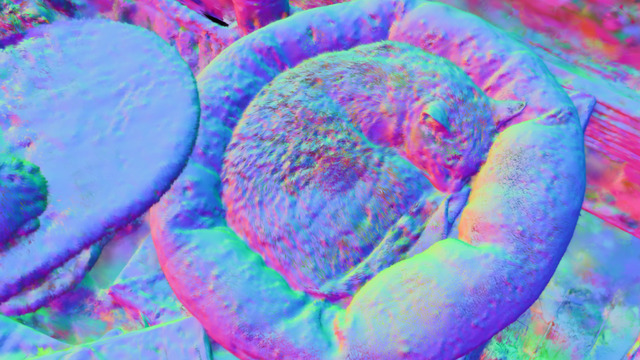
\includegraphics[width=\linewidth]{images/normals/sirius1_normals_52_bis.jpg}
  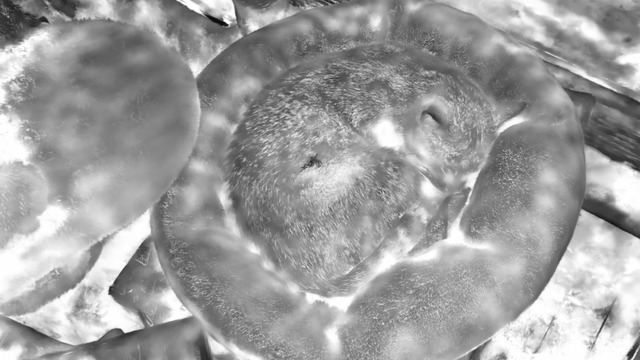
\includegraphics[width=\linewidth]{images/frosting_size/sirius1_size_52_ter.jpg}
  \end{subfigure}
  %
  \hfill
  %
  \begin{subfigure}{0.155\linewidth}
  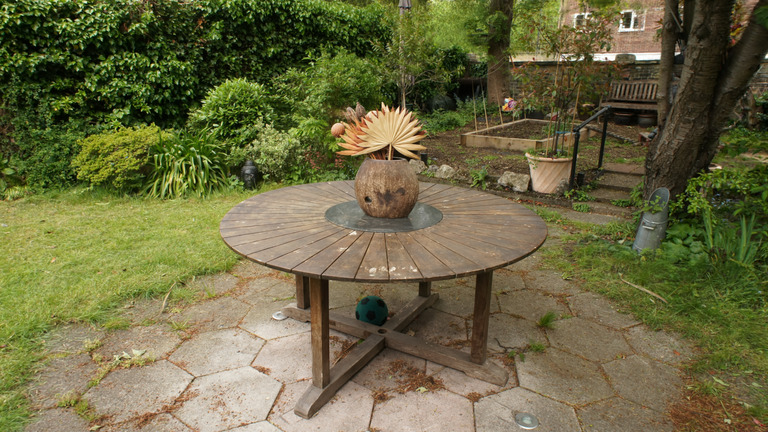
\includegraphics[width=\linewidth]{images/renders/garden_rgb_31.jpg}
  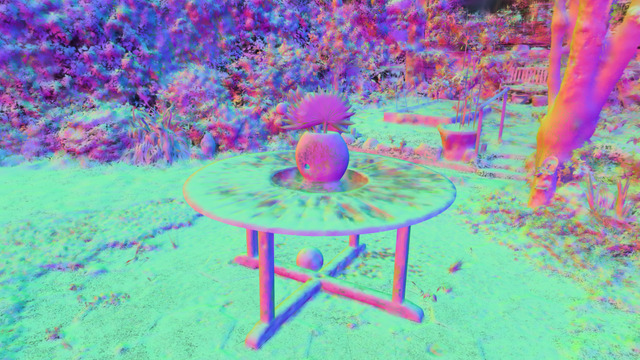
\includegraphics[width=\linewidth]{images/normals/garden_normals_31bis.jpg}
  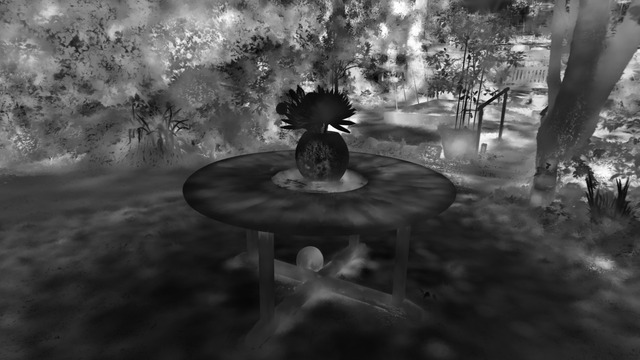
\includegraphics[width=\linewidth]{images/frosting_size/garden_size_31bis.jpg}
  \end{subfigure}
  %
  \hfill
  %
  \begin{subfigure}{0.155\linewidth}
  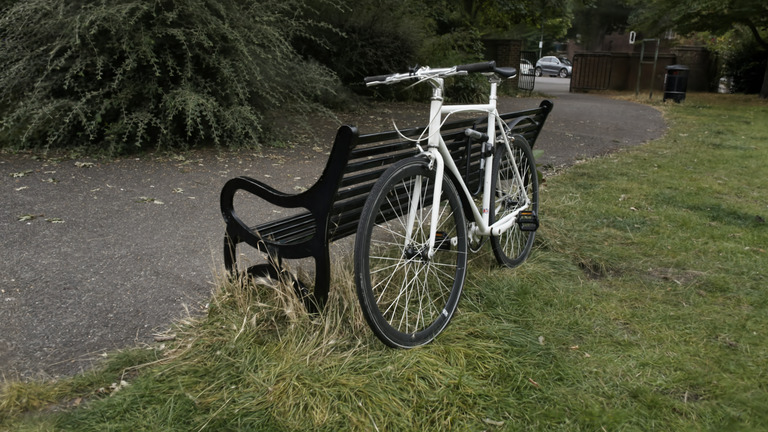
\includegraphics[width=\linewidth]{images/renders/bicycle_rgb_52.jpg}
  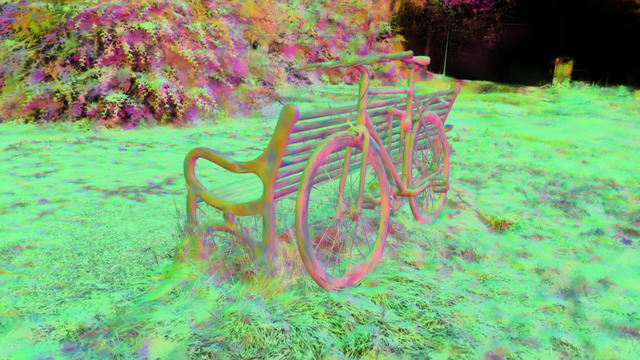
\includegraphics[width=\linewidth]{images/normals/bicycle_normals_52bis.jpg}
  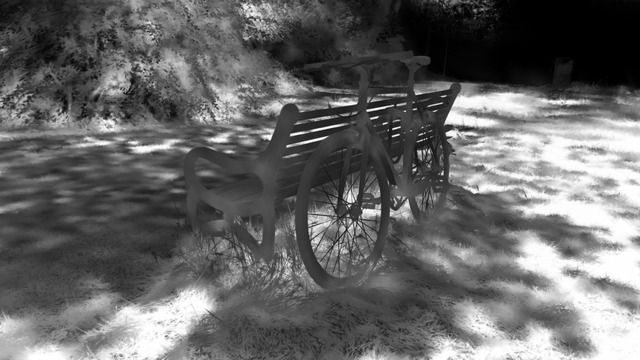
\includegraphics[width=\linewidth]{images/frosting_size/bicycle_size_52bis.jpg}
  \end{subfigure}
  %
  \caption{
  \textbf{Rendering complex scenes with Frosting.} First row: Renderings, Second row: recovered normal maps, Third row: estimated Frosting thickness. Note that the Frosting is thick on fuzzy materials such as the hair and the grass, as expected, and very thin on flat surfaces such as the table on the fourth column.
  }
  \label{fig:frosting-renders}
\end{figure}


\subsection{Frosting Optimization}

Once we constructed the outer and inner bounds of the Frosting layer, we initialize a densified set of Gaussians inside this layer and optimize them using 3DGS rendering loss as the unconstrained Gaussians. To make sure the Gaussians stay inside the frosting layer during optimization, we introduce a new parameterization of the Gaussians. Moreover, this parameterization will make possible to 
easily adjust the Gaussians' parameters when editing the scene.


\subsubsection{Parameterization.} Let us consider a triangular face of the base mesh $\calM$, with vertices denoted by~$\vec{v}_0, \vec{v}_1$, and~$\vec{v}_2$ and their corresponding normals~$\vec{n}_0, \vec{n}_1$, and~$\vec{n}_2$. After extracting inner and outer shifts from unconstrained Gaussians, we obtain six new vertices $(\vec{v}_i+\innershift_i \vec{n}_i)_{i=0,1,2}$ and $(\vec{v}_i+\outershift_i \vec{n}_i)_{i=0,1,2}$ that respectively belong to the inner and outer bounds of the frosting.
%
Specifically, these six vertices delimit an irregular triangular prism. We will refer to such polyhedrons as ``prismatic cells''. 
%
We parameterize the 3D mean~$\mu_g\in \IR^3$ of a Gaussian~$g \in \calG$ located inside a prismatic cell with a set of six barycentric coordinates split into two subsets~$(b_g^{(i)})_{i=0,1,2}$ and $(\beta_g^{(i)})_{i=0,1,2}$, such that 
%
\begin{equation}
    \mu_g = \sum_{i=0}^2 \left(
    b_g^{(i)} \left(\vec{v}_i+\outershift_i \vec{n}_i\right) +
    \beta_g^{(i)} \left(\vec{v}_i+\innershift_i \vec{n}_i\right)\right) \> ,
    \label{eq:barycentric-coordinates}
\end{equation}
%
with barycentric coordinates verifying $\sum_{i=0}^2 ( b_g^{(i)}+\beta_g^{(i)}) = 1$.
%
Using barycentric coordinates enforces Gaussians to stay inside their corresponding prismatic cell, and guarantees the stability of our representation during optimization.
%
In practice, we apply a softmax activation on the parameters to optimize to obtain barycentric coordinates that sum up to 1. 

\subsubsection{Initialization.} For a given budget $N$ of Gaussians provided by the user, we initialize $N$ Gaussians in the scene by sampling $N$ 3D centers $\mu_g$ in the frosting layer. Specifically, for sampling a single Gaussian, we first randomly select a prismatic cell with a probability proportional to its volume. Then, we sample random coordinates that sum up to 1. 
This sampling allows for allocating more Gaussians in areas with fuzzy and complex geometry, where more volumetric rendering is needed. However, flat parts  in the layer may also need a large number of Gaussians to recover texture details. Therefore, in practice, we instantiate $N/2$ Gaussians with uniform probabilities in the prismatic cells, and $N/2$ Gaussians with probabilities proportional to the volume of the cell.

We initialize the colors of the Gaussians with the color of the closest Gaussian in the unconstrained representation. However, we do not use the unconstrained Gaussians to initialize opacity, rotation, and scaling factors, as in practice, following the strategy from 3DGS~\cite{kerbl3Dgaussians} for these parameters provides better performance: 
We suppose the positions and configuration of the Gaussians inside the Frosting layer are already a good initialization, and resetting opacities, scaling factors and rotations helps Gaussians to take a fresh start, avoiding a potential local minimum encountered by previous unconstrained Gaussians.

Our representation allows for a much better control over the number of Gaussians than the original Gaussian Splatting densification process, as it is up to the user to decide on a number of Gaussians to instantiate in the frosting layer. These Gaussians will be spread in the entire frosting in a very efficient way, adapting to the need for volumetric rendering in the entire scene.

\subsubsection{Optimizing the Gaussian Frosting.} We reload the unconstrained Gaussians and apply our method for computing the inner and outer bounds of the Frosting. Then, for a given budget of $N$ Gaussians, we initialize $N$ Gaussians in the Frosting and optimize the representation while keeping the number of Gaussians constant. Note that compared to Vanilla 3DGS, this allows to control precisely the number of Gaussians.


\subsubsection{Editing, Deforming, and Animating the Frosting.} When deforming the base mesh, the positions of Gaussians automatically adjust in the frosting layer thanks to the use of the barycentric coordinates. 
%
To automatically adjust the rotation and scaling factors of the Gaussians, we propose a strategy different from the surface-based adjustment from SuGaR: In a given prismatic cell with center $\vec{c}$ and vertices $\vec{v}_i$ for $0\leq i<5$, we first estimate the local transformation at each vertex $\vec{v}_i$ by computing the rotation and rescaling of the vector $(c - \vec{v}_i)$. 
%
Then, we use the barycentric coordinates of a Gaussian $g$ to compute an average transformation at point $\mu_g$ from the transformation of all 6 vertices, and we adjust the rotation and scaling factors of $g$ by applying this average transformation. 
%
Please note that the spherical harmonics are also adjusted in practice, to ensure the consistency of the emitted radiance depending on the averaged rotation applied to the Gaussian.
%
We provide more details about this automatic adjustment of Gaussian parameters in the supplementary material.